\chapter{Results - Implementation}

\label{ch:implementationresults}

blablabla dass die das ergebnis von --langem-- rumprobieren sind

%############################################################################################
\section{Possible vectors}
%############################################################################################

\label{ch:thevectors}

%-progressvec (progress, laptime, lapcount, validvec)
%-speedsteer (motortorques, steerangle, velocity, fRightDirection, velocity of perpendiculars, angle, speedinstreetdir, speedintraversedir, cuvinessbeforecar)
%-carstatusvec (longitutinal and latidutialn slip for each tire)
%-centerdist, als vector
%-waldistvec (direction the car faces, steers, moves..... and directiont the street goes (each longsighted and shortsighted from car and streetmiddle)
%-lookahead-vector
%-delta und feedback
%-actual action (possibly overwritten)
%-both vision-vectors

\term{Possible Vectors} refers to all information the game streams over its socket to the agent. While most of this information will be used to make up an agent's state, the vectors also provide information about if the game must be reset as well as information to calculate the reward from. This information is collected in Unity in the function \codefunc{GetAllInfos()}, and converted into a namedtuple-wrapper called \codeobj{Otherinputs}, specified in \filename{read\_supervised.py}. In this section, I provide an overview of those vectors and their meaning in the game. I refer to the individual possible vectors by the name used in \codeobj{Otherinputs}.

\paragraph{ProgressVec} This vector contains information about the current progress of the car on the track, which consists of the actual progress in percent, the time the car needed for the current lap so far, the number of the current lap, as well as the flag if the round is still valid (which is the case if the car did not leave the street yet).

\paragraph{SpeedSteer} In this vector, information about the car's velocity and its steer angle is encoded. It consists of the following values:

\renewcommand{\arraystretch}{1.3}
\begin{flushleft}
	\begin{tabular}{>{\em}p{2.9cm} p{\textwidth-3.8cm}} 
		RLTorque & The motor torque applied to the left back tire\\
		RRTorque & The motor torque applied to the right back tire\\
		FLSteer & The steering angle of the front left tire\\
		FRSteer & The steering angle of the front right tire\\
		velocity & The velocity of the car as scalar independent of directions\\
		rightDirection & A boolean value if the car moves into the intended direction\\
		velocityOfPerpendiculars & \hspace*{0.8cm} The velocity of the orthogonal projection of the car onto the center of the street\\ %TODO see sectionbalabla, wo ich DOCH die definition von perpendicular einführen werde
		carAngle & The car's angle (in degrees) in relation to the street's direction\\
		speedInStreetDir & The car's velocity into the street's direction (calculated using the dot-product between the car's velocity-vectors and the direction-vector of the street at the car's current position)\\
		speedInTraverDir &  The car's velocity into the orthogonal of the street's direction\\
		CurvinessBeforeCar & A measure of the curvature of the street immediately ahead of the car ($CurvinessBeforeCar \in [0,1]$, where a value of zero corresponds to a straight street)\\	
	\end{tabular}
\end{flushleft}

\paragraph{StatusVector} This vector contains eight values, corresponding to the forward slip and sideways slip of each of the car's tires, using a function provided for Unity's \codeobj{WheelCollider}-object. The more the car slips, the smaller the impact of movement commands. The current slip-values are presented in the GUI of the game (and can be seen behind annotation \textbf{R} in figure~\ref{fig:aidriveshot}).

\paragraph{CenterDist and CenterDistVec} The \emph{CenterDist} corresponds to the car's orthogonal distance to the street's center, as calculated in \colorbox{red}{where} (also visually represented in the car's GUI, behind annotation \textbf{N} in figure~\ref{fig:aidriveshot}).
The \emph{CenterDistVec} contains the same information presented in another way: It is a vector of length 15, where the middle element corresponds to the car's longitutional position. The other elemnts correspond to points with regular distances to the car's left and right. The value of each respective element is calculated using the reversed distance between this position and the longitudional center of the street. The content of this vector is visually represented behind annotation \textbf{M} in figure~\ref{fig:aidriveshot}.

\paragraph{WallDistVec} This vector contains seven values, corresponding to the car's distance to the wall along a certain ray. It does not contain the closest distance to the wall -- because this value is already represented by the CenterDist. As the wall has always a fixed distance from the street's center (with an absolute value of five), the distance to the closest wall can be calculated as $5 - abs(CenterDist)$. 
For the calculation of the \emph{WallDistVec}, several rays are casted from the car's (or the perpendicular's) position into a particular direction. Returned is then the distance from their respective origin and their first intersection with a wall. The vector contains seven values, using rays with different origins and different directions. In the following table, I provide an explanation of each of those values, while figure~\ref{fig:walldistvec} in appendix~\ref{AppendixB} visually represents these rays. The respective color is mentioned in the table.
\renewcommand{\arraystretch}{1.3}
\begin{flushleft}
	\begin{tabular}{p{0.5cm} p{2cm} p{2.4cm} p{\textwidth-6.45cm}} 
		\# & color in \ref{fig:walldistvec} & origin & direction \\
		\hline
		1 & \textcolor{black}{black} & car's center & direction the car faces \\
		2 & \textcolor{magenta}{magenta} & car's center & direction the car steers\\	
		3 & \textcolor{red}{red} & car's center & direction the car moves\\	
		4 & \textcolor{black}{white} & car's center & short-sighted direction of the street (calculated as the vector between the closest \codeobj{anchorVector} behind the car and the closest one before the car) \\		
		5 & \textcolor{yellow}{yellow} & perpendicular & short-sighted direction of the street (calculated as the vector between the closest \codeobj{anchorVector} behind the car and the closest one before the car) \\
		6 & \textcolor{blue}{blue} & car's center & long-sighted direction of the street (calculated as the vector between the closest \codeobj{anchorVector}  to the car and the one 5 in advance) \\
		7 & \textcolor{gray}{gray} & perpendicular & long-sighted direction of the street (calculated as the vector between the closest \codeobj{anchorVector}  to the car and the one 5 in advance) \\
	\end{tabular}
\end{flushleft}

\paragraph{LookAheadVec} This vector corresponds to the course of the street ahead of the car. It is a vector consisting of 30 elements, corresponding to regularly spaced \codeobj{anchorVector}s, starting at the position of the car, following the direction of the street. The value at each position $i$ of this vector corresponds to the angle between the direction of the street at position $i$ and the direction at position $i+1$. In other words, if the street makes a shart turn 4 units ahead of the car, then element $3$ will contain a high value. The angle is measured in degrees. A graphical representation of this vector can be seen behind annotation \textbf{N} in figure~\ref{fig:aidriveshot}.

\paragraph{FBDelta} This vector consists of two values, namely \emph{Feedback} and \emph{Delta}. The Feedback-value is the temporal difference of how long the car needed for a specific section of the course (constrained via the closest \codeobj{anchorVector}s of the car) in the current process in comparison to the time needed in the fastest lap so far. The Delta-value is the absolute difference in time needed for the entire lap so far.

As both of these values are only useful in relation to the time needed for the fastest lap, it must be ensured that this does not change during training. For that, The file \filename{AiInterface.cs} contains in its class \codeobj{Consts} a flag \codeobj{lock\_fastestlap\_in\_AIMode}. Note however, that even if this flag is set, the values of \emph{FBDelta} could at most be used to calculate the agent's reward and not as part of its state.

\paragraph{Action} This is a three-dimensional vector corresponding to the actual action the environment recorded. While the agent knows what action it provided, it could be manually overwritten (after the press of \keystroke{H}) -- which is why the agent stores this vector in its replay memory instead of the action it would have performed otherwise.


\paragraph{Mini-maps} While the content of the mini-maps is not contained in the namedtuple \codeobj{Otherinput}, their value is transmitted from the game just like the other vectors. In the current implementation, both cameras have a resolution of $30\times45$ pixels, where one camera is $15$ units away of the car, and the other one $75$ units, which means that the former provides a smaller but more detailed view of the car. The closer camera is mostly referred to as $vvec2$, whereas the other one is denoted $visionvec$ or $vvec$.\\

As a working game was already provided by \leon of this thesis, so were some of these vectors, namely the calculation of FBDelta, LookAheadVec, CenterDist and CenterDistVec, as well as many elements necessary to compute many of the other ones. 
It is worth noting that most \term{possible vectors} are normalized after loading, according to (in part estimated) minimal- and maximal values, such that all their values in [0,1]. The corresponding \codeobj{MINVALS} and \codeobj{MAXVALS} are defined in \filename{read\_supervised.py}

%############################################################################################
\section{Implemented Models}
%############################################################################################

Within the context of this thesis, two different models were developed that can be used for agents to learn and play the given game: a \keyword{Double Dueling Deep-Q-Learning} model, specified in the class \codeobj{DDDQN\_model} in \filename{models/dddqn.py}\footnote{\url{https://github.com/cstenkamp/BA-rAIce-ANN/blob/master/models/dddqn.py}} as well as a \keyword{Deep Deterministic Policy Gradient} model, specified in \codeobj{DDPG\_model} in \filename{models/ddpg.py}\footnote{\url{https://github.com/cstenkamp/BA-rAIce-ANN/blob/master/models/ddpg.py}} Both models learn via temporal differences and are in detail explained in chapters~\ref{ch:DQN}ff and \ref{ch:ddpg}, respectively. 

Both models can take two-dimensional as well as one-dimensional input and return outputs corresponding to the action that needs to be taken, which are three real numbers. One has to be aware though that while a DDPG-model can naturally return such, a DQN-model only works for discrete actions. Because it was developed with DQN-models in mind, the \codeobj{AbstractAgent} contains functions to \codefunc{discretize} the action-value returned by the game to a one-hot vector to be used by the model, as well as functions to \codefunc{dediscretize} a one-hot vector from the model that can be used by the environment. It is obvious, that discretizing actions has severe disadvantages: If the discretization is very fine-grained, the action-space becomes intractably big due to a combinatorial explosion (the \textit{curse of dimensionality}), whereas if a discretization is coarse, much of the information is lost and precise steering becomes impossible. A further downside of discretizing actions into one-hot vectors is, that it limits the design space of exploration strategies, as information about similiarity of actions is lost and only uninformed $\epsilon$-greedy remains possible.

In the \term{Drive}-mode of the game, throttle and steering are both binary, but it is still possible for Users to drive the course well. Because of that, it was decided to keep steering and throttle binary in this mode as well, to reduce the dimensionality of discretization. Further, simultaneous activation of throttle and brake was forbidden. Because of these design choices, an action for a DQN-model is a one-hot vector of the size \codeobj{3*conf.steering\_steps}, with steering\_steps set to 7 in the current version. If an agent does not need to discretize actions, it must overwrite the method \codefunc{getAction(gameState)}.\\

\noindent While the learning technique differs in both implemented models, both implement the interface provided in figure~\ref{fig:modelsInt}, such that the functions relevant for the agent are accessible in the same way. An UML-diagram of most of their functions as well as the interface is given in figure~\ref{fig:modelssmall}. 

\begin{figure}[h]
	\centering 
	\includegraphics[width=\textwidth]{uml_diagrams/models_inText2.2}
	\caption{UML-diagram of the two given models as well as the interface both of them implement}
	\label{fig:modelssmall}
\end{figure}

Both implemented models provide the possibility to load and save a model from/to the harddisk unsing TensorFlow's saver-class. If a model is loaded in the \codeother{isPretrain}-mode, it can be saved to file and loaded again such that it is usable. If the model is saved, the information about its already performed numbers of inferences and learning-steps are saved within TensorFlow as well. When a model is saved, it saves into the directory \codeobj{conf.pretrain\_checkpoint\_dir} if the respective flag is set, and \codeobj{conf.checkpoint\_dir} else. When loading a model (in \codefunc{initNet(load)}), the \codefunc{load}-parameter specifies if the model should be loaded from the pretrain-directory, the non-pretrain-directory or none at all.


While both models are implemented to be used by the described agent and in the described situation, they are general models for reinforcement learning -- and are as such usable to learn reasonable policies in any task described as markov decision process. To show the generality of the implemented models, a file \filename{gym\_test.py}\footnote{\url{https://github.com/cstenkamp/BA-rAIce-ANN/blob/master/gym\_test.py}} is provided. In this file, the implemented \codeobj{model}s are used to solve arbitrary \term{openAI-gym}-tasks. As the program flow of the interaction with a gym-environment differs to that one of the implemented program, the file contains specialized definitions of \codeobj{agent}, \codeobj{config} and \codeobj{memory} to work with the API-schema of \term{gym}. As \term{gym}-environments explicitly define \codeobj{terminal} and \codeobj{reward}, the \codeobj{agent} must for example not work with the \codeobj{gameState}, but contains only methods using the immediate \codeobj{agentState}. -- the way how an agent accesses its model is however equal to the agents for the given game. The \filename{gym\_test.py} can be used to test if a model is functional -- if a model works on several gym-tasks, it can be assumed that it is implemented correctly. Having such a method at hand is very handy during the implementation of reinforcement-learning agents, as it provides a reliable method to check where the reason for any errors may lie. Both implemented models were successfully tested on several tasks each\footnote{Note however, that using other gym-environments than the ones on which was tested (\codeobj{Pendulum-v0}, \codeobj{FrozenLake-v0}, \codeobj{MountainCar-v0} and \codeobj{CarRacing-v0}) may require implementing specific exploration or preprocessing techniques. Note further, that some environments can only be solved with models that allow for continuous action-spaces.}.
\colorbox{red}{https://gym.openai.com/envs/CarRacing-v0}

In the following two sections, I will at first explain the DQN-model and afterwards the DDPG-model. Note that both models are used in multiple agents each. The amount of input-values may just differ from agent to agent, and the presented network architecture is specific to one of the implemented agents, which will be explained in a following section.


\subsection{DQN-model}

\colorbox{red}{decaying LR is implemented but should only be used in svtrain}

The class \codeobj{DDDQN\_model} \term{has} two \codeobj{DuelDQN}s, which are Deep Convolutional Neural Networks with Dueling Architectures, specified as computational graph using TensorFlow -- one of them being its online network, and the other the target network. The \codeobj{DDDQN\_model} combines then for the learning method of Double-Q-Learning (as detailed in section~\ref{ch:DQN}ff as well as appendix~\ref{AppendixA}) in its method \codefunc{q\_train\_step}. 

The provided DQN-model can however not only learn via Q-learning, but can also be trained supervisedly. For that, it also specifies the function \codefunc{sv\_train\_step}. This method can only be called if \codeobj{isPretrain} and learns directly on its target network. For that, the used \codeobj{DuelDQN}s must provide a TensorFlow-placeholder for the target-action. An agent that pretrained supervisedly however should not subsequently be used for reinforcement learning. An explanation for that will follow in the next chapter.

It was mentioned before that the model incorporates hard-coded domain-specific knowledge. Next to the ban of simultaneous braking and steering as action, the model explicitly forbids actions that do not accelerate the car if it is standing. As already mentioned, part of the \codeobj{agentState} is a \codeobj{stands\_input}, which the method \codefunc{getAgentState} sets to \codeobj{true} if the car's velocity is below a certain value. The model has consistently as \codeobj{stands\_input}, which expects such a boolean value. Note that the model's \codefunc{make\_inputs} also actively sets this value to \codeobj{true} if the car stood up to a specified number of inferences before the current one. If this value is \codeobj{true} and the respective option \codeobj{conf.use\_settozero} is set to \codeobj{true}, then the model sets in the function \codefunc{settozero} all q-values of actions that do not include accelerating the car to a large negative value. As a DQN-based model selects its actions using a \textit{greedy} strategy, it always selects the action with the highest Q-value -- which is now the maximum of all Q-values that include the action of accelerating the car. Note however, that the model's \codeobj{stands\_input} is only set to \codeobj{true} in inferences, and not in learning-steps.

The network architecture of the two \codeobj{DuelDQN}s that the agent uses is described in the next section. Note that a \codeobj{DuelDQN} is a particular class \term{know}n to the agent. All TensorFlow-Layers, inputs, outputs as well as a \codeobj{saver} and certain collections can be accessed from the \codeobj{DDDQN\_model}. As explained in chapter~\ref{ch:DQN}, the use of both online-network to train on as well as target-network to sample experiences from is necessary for adequate performance. As suggested by \cite{lillicrap_continuous_2015}, the implementation of this DQN uses \textit{soft target-updates}, meaning that after every \codefunc{q\_train\_step} the relevant weights of the target-network are moved by a factor $0 < \tau \ll 1$ into the direction of the online-network. To do so, both networks store their collection of trainable variables,  \codeobj{trainables}. The respective assignment operations are added to the computational graph as \codeobj{smoothTargetNetUpdate}, specified in the model's \codefunc{\_\_init\_\_}. After initializing a model or loading it from a file, a similar assignment operation is performed to ensure that both networks are equal.

\subsubsection{Network architecture}

An overview of the general network architecture, as used by the \codeobj{dqn\_rl\_agent}, is provided in figure~\ref{fig:dqn_graph}. Note however that the actual architecture differs in other agents, as it depends on the agent's configuration of \term{features}. As some agents do not use the minimaps as input, their implementation therefore does not use any of the convolutional layers from the upper line of the figure. When initializing a \codeobj{DuelDQN}, a reference to the agent is passed, such that the network knows how many input and output-neurons to specifiy.

\begin{figure}[h]
	\centering 
	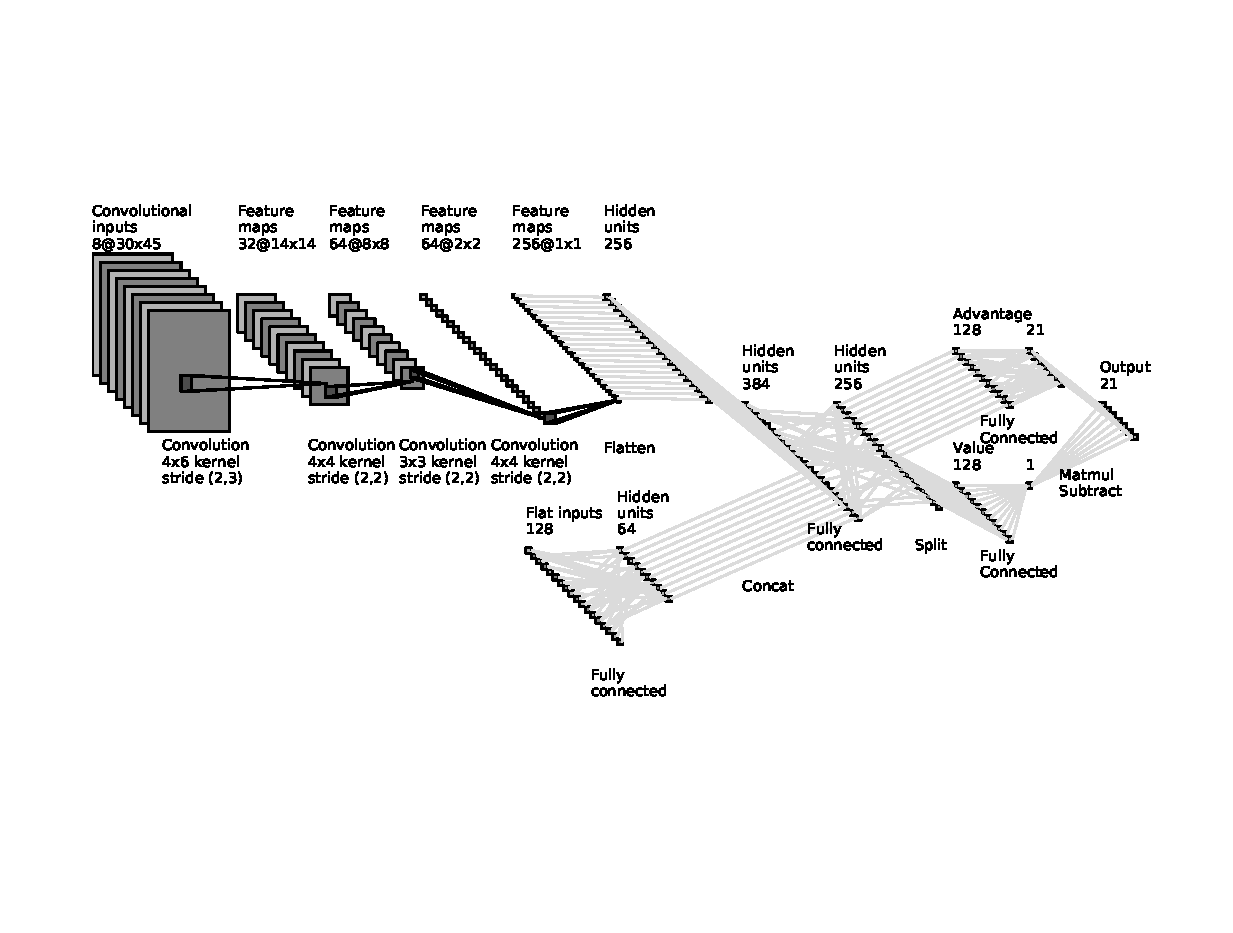
\includegraphics[trim={1.22cm 3.4cm 1.15cm 3cm},clip,width=1.05\textwidth]{draw_convnet/dqn}
	\caption{The used convolutional DQN with a dueling architecture}
	\label{fig:dqn_graph}
\end{figure}

If convolutional input is specified, four convolutional layers layers processes the input to 256 feature-maps of size $1 \times 1$, which can subsequently be flattened to a one-dimensional layer. Note that there are no pooling layer in between convolutional layers. As suggested by \cite{springenberg_striving_2014}, pooling leads to a loss of localization information and can be discarded in favor of a larger \term{stride} in the convolutional layers.

While the two-dimensional \codeobj{conv\_inputs} are processed with convolutional layers, the \codeobj{ff\_inputs} are connected with a dense layer to a hidden layer of variable size. This layer is concatenated to the flattened output to the convolutional layer, the result of which is densely connected to another hidden layer of 256 neurons. This layer is then, following the dueling architecture from \cite{wang_dueling_2015}, split into a separate \codeobj{Advantage stream} and \codeobj{Value stream}. While the value stream is fully connected to one hidden layer (corresponding to the state-value), the advantage ends in one output neuron for action, which is 21 in the current implementation. The advantage stream and value stream are finally combined (as described in section~\ref{sec:dueling}) to yield 21 output neurons, corresponding to one Q-value for every action in the provided state.

Informal search led to the selection of the rectified non-linearity (\codeobj{tf.nn.relu}) as activation function as well as Adam\cite{kingma_adam:_2014} as optimizer. All weights of this network are initialized around zero (or slightly higher, to prevent \term{dead neurons} in combination with the relu activation-function) with only a very small standard deviation ($10^{-20}$ up to $10^{-3}$), as doing otherwise showed to impair the agent's performance at start.

In the current implementation, the DQN-model does not perform \term{batch normalization}\cite{ioffe_batch_2015}, as it showed to decresed the agent's performance. The functions \codefunc{convolutional\_layer} and \codefunc{dense}, which are used to initialize the layers, wrap respective TensorFlow-functions and can be found in \filename{utils.py}\footnote{\url{https://github.com/cstenkamp/BA-rAIce-ANN/blob/master/utils.py}}.

The final structure of this network was the subject of much experimentation. Any used hyperparameter that does not correspond to its counterpart in \cite{mnih_human-level_2015} or \cite{wang_dueling_2015} is the result of informal search, showing the best performance so far. This does by any means not mean that the parameters are optimal. Using this structure, the network performed reasonably well on given openAI gym-tasks, as explained earlier in this chapter.


\subsection{DDPG-model}

\colorbox{red}{Agents that use the DDPG-model must overwrite the functions makenetusableaction and getAction, add make\_noisy and overwrite randomaction, as they likely use policyaction + noise instead of epsilon-greedy}

A DDPG-model must incorportate four ANNs to work correctly: an online- and a target version of both \codeobj{actor} and \codeobj{critic}, as found by \cite{lillicrap_continuous_2015}.  While the online networks will be used for online predictions and will be updated at every timestep, the target networks will be used for determining the directions in which the online networks should be updated. The given implementation of the \codeobj{DDPG\_model} thus \term{has} an actor and a critic, which in turn have two \codeobj{actorNet}s or \codeobj{criticNet}s, respectively. If the \codefunc{save()}-method of \codeobj{DDPG\_model} is called, it calls the respective functions of actor and critic, which save their individual variables individually. Because of that, the same critic could be used for different actors or vice versa. The information about the numbers of current inferences and others is saved in and loaded from the actor.

As the \codeobj{DDPG\_model} \term{has} \codeobj{actor} and \codeobj{critic}, it can access all their values and methods. If it accesses any of these, it specifies as argument if it wants them to internally sue their online- or target network. To update the target network, both actor and critic provide respective methods.

It is not possible to use the same network structure as used in the \codeobj{DQN\_model} in any network of the \codeobj{DDPG\_model}. The actor returns a continuous values which correspond directly to the action instead of a \term{softmax}-distribution over possible discrete actions. The critic needs, in contrast to the DQN-architecture, the actions as additional input to return one single Q-value. It is obvious, that the \term{dueling architecture} cannot be adopted for the DDPG-critic.

In its \codefunc{q\_train\_step}-method, the \codeobj{DDPG\_model} trains both its actor and its critic by calling their respective methods -- the theoretical basis of this learning step is explained in section~\ref{ch:ddpg} and appendix~\ref{ap:ddpg} compares the source-code to the Pseudocode given in \cite{lillicrap_continuous_2015}. It is possible in TensorFlow to extract the \term{gradients} of a complete graph of computations, namely the critic. While normally TensorFlow minimizes losses via an optimizer (and also does so in the critic), it also allows the possibility to \codefunc{apply\_gradients}, which optimizes all elements of its respective computation graph into the direction of the supplied values. 

As the actor only needs the critic's gradients once, these can simply be passed into its \codeobj{feed\_dict}. Besides this interaction, actor and critic can be implemented completely independent of each other. In the following section, I will describe the network structure of both of them individually. It is worth noting, that this model supports the usage of \term{TensorBoard}, and saves a summary of all its variables in a preset interval of update-steps.

\subsubsection{Network architecture}

\paragraph{Critic}

The actual computational graph of the network the \codeobj{critic} uses is specified in an extra class. In contrast to the \codeobj{DQN\_model}, it was decided to use a different class for agents that use convolutional input than for agents which do not. Informal testing it showed that the \codeobj{DDPG\_model} appears to be less forgiving to changes of its network structure. This means, that the \codeobj{criticNet} uses a \codeobj{conv\_criticNet} if \codeobj{agent.usesConv} and a \codeobj{lowdim\_criticNet} else.

The critic gets as input a state and an action, and returns an estimate of the respective state-action value \term{Q}. In contrast to the model of a DQN, it gets both of these as input and returns a single value. Like a DQN however, it is trained using temporal differences, requiring a better estimate of each Q-value to update its parameters. As however only the online network is updated this way (whereas the target-network receives smooth updates, as explained above), the \codeobj{placeholder} to hold these is specified in the class \codeobj{Critic}, not in one of its used networks.



\colorbox{red}{beim actor noch die settozero-funktion, und wie sie anders ist!!!}
\colorbox{red}{nochmal dass alle near zero initialized werden}
\colorbox{red}{reader soll ins ddpg-paper für die precise hyperparams gucken}

\begin{figure}[h]
	\centering 
	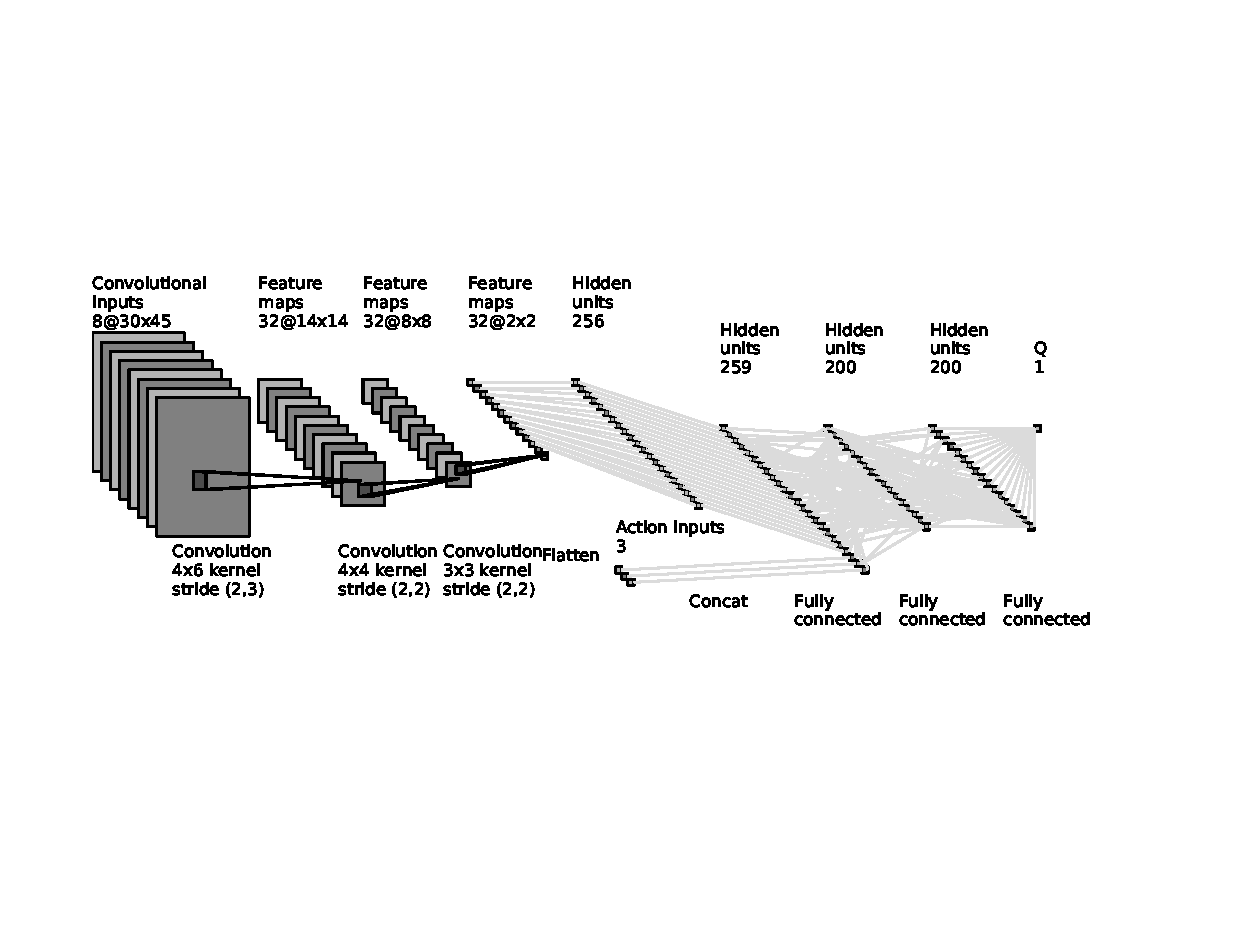
\includegraphics[trim={1.22cm 4.6cm 2cm 3cm},clip,width=1.05\textwidth]{draw_convnet/critic-2d}
	\caption{Convolutional critic}
	\label{fig:2dcrit}
\end{figure}

\begin{figure}[h]
	\centering 
	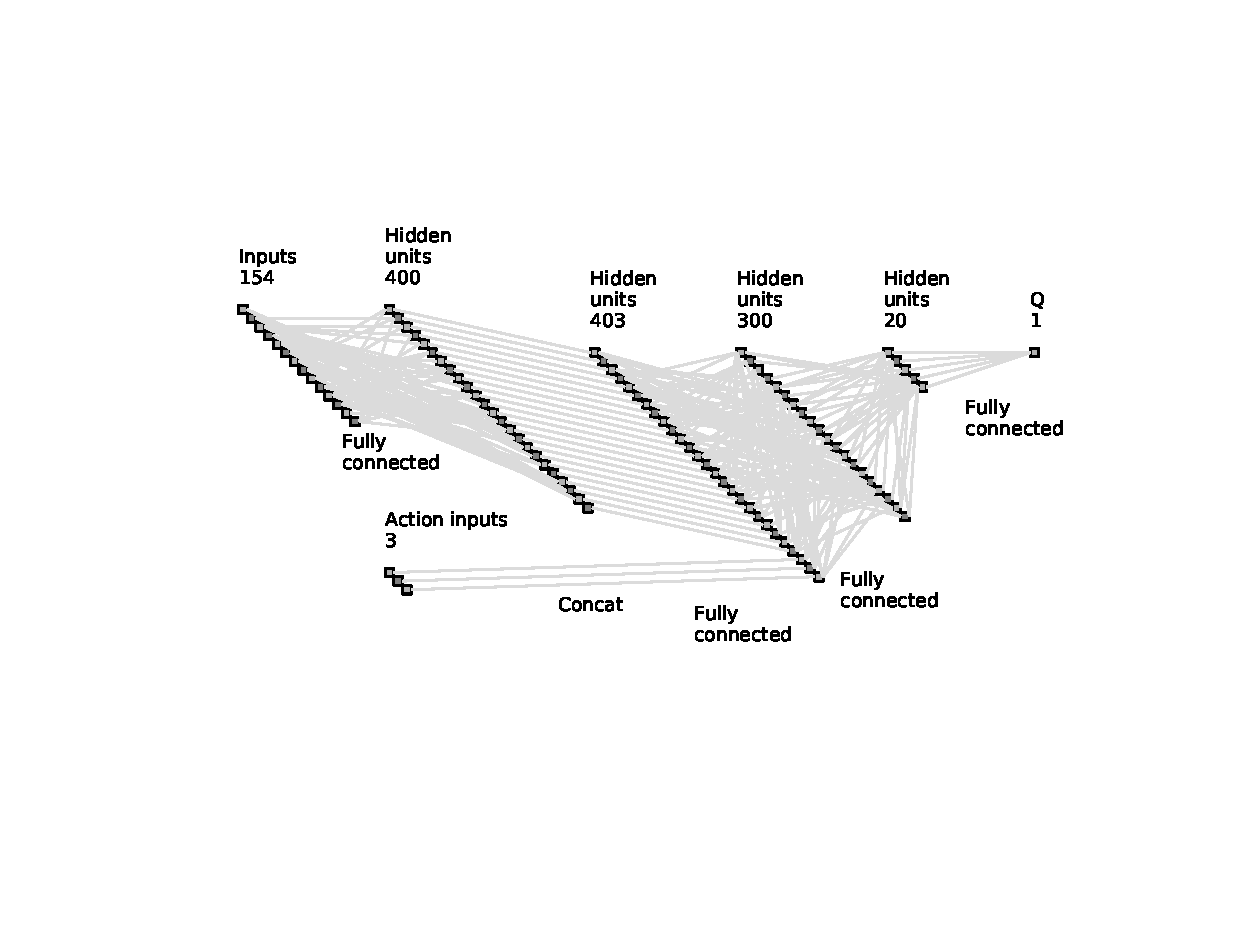
\includegraphics[trim={3.7cm 4.4cm 2cm 3cm},clip,width=1.05\textwidth]{draw_convnet/critic-lowd}
	\caption{Low-dimensional critic}
	\label{fig:lowcrit}
\end{figure}

\begin{figure}[h]
	\centering 
	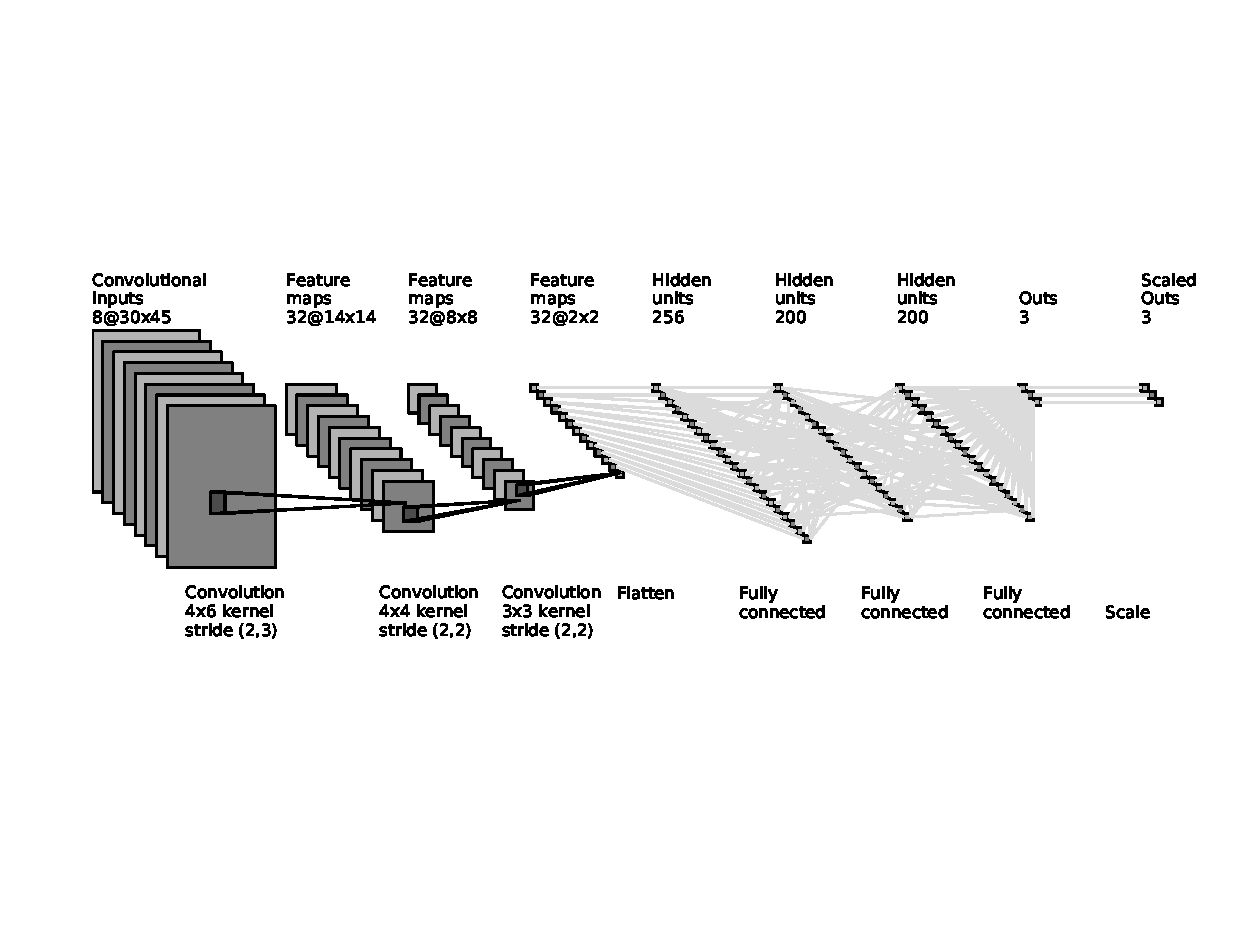
\includegraphics[trim={1.22cm 5.03cm 0.4cm 3cm},clip,width=1.05\textwidth]{draw_convnet/actor-2d}
	\caption{Convolutional actor}
	\label{fig:2dact}
\end{figure}

\begin{figure}[h]
	\centering 
	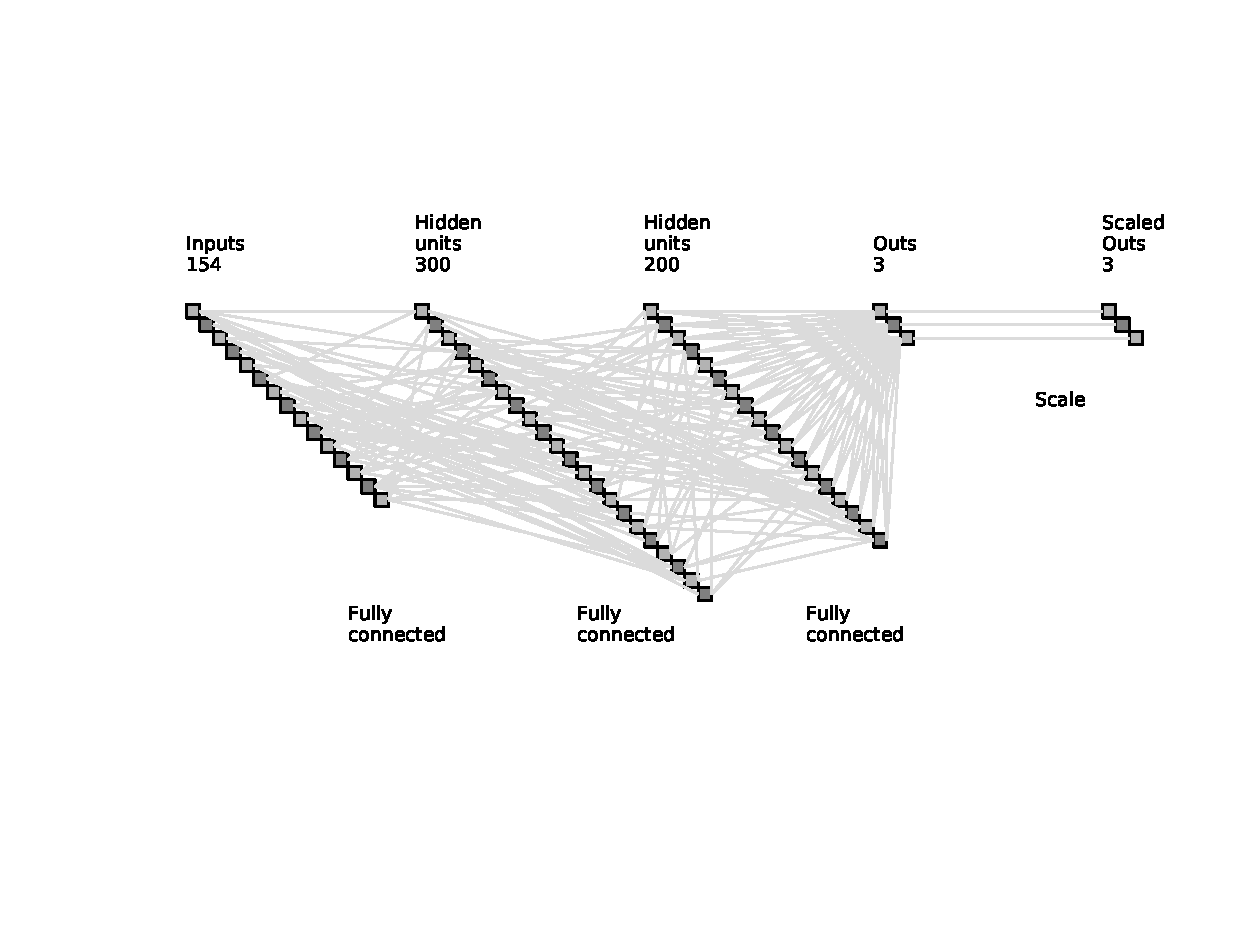
\includegraphics[trim={2.7cm 4.2cm 0.8cm 3cm},clip,width=1.05\textwidth]{draw_convnet/actor-lowd}
	\caption{Low-dimensional actor}
	\label{fig:lowdact}
\end{figure}

In a hybrid ANN (having both 2D and 1D input), four convolutional layers calculate an abstract representation of the two-dimensional inputs, which is flattened into a hidden layer consisting of 256 Units. The one-dimensional input are connected via a dense layer to another hidden layer of 64 units. These two layers are then concatenated to form a layer of 384 hidden Units, which is densely connected to a further hidden layer, which splits into an advantage and a value stream as proposed by \cite{wang_dueling_2015}. While the advantage stream ends in a layer with one unit for each action, the value-stream has one output. In the very last layer of the network, the advantage and value stream are combined into the final output layer, providing a separate Q-value for each action.

\colorbox{red}{batchnorm auf jedem layer separately}
\colorbox{red}{uses tf.layers.dense und slim.conv2D}
\colorbox{red}{stores summaryOps für tensorboard}
-sets if both brake and throttle are high one of them at random to a low value (if not accplusbreak)
-sets brake-values to zero and throttle to a bit if carstands and the option is set

No pooling, nur stride

There are two different models implemented in this project: 


blablabla überleitung dass ich jetzt erst das eine dann das andere erläutere

1. dqn-algorithm
- anzahl layer, Batchnorm, doubles dueling
- clipping wieder rein, reference auf das dueling
- grundsätzlich gegen batchnorm entschieden, siehe reddit post
- MIT GRAFIK
- Adam und tensorflow quoten, siehe zotero
2. ddpg
- anzahl layer, Batchnorm
- MIT GRAFIK

-mo
-schöne grafik.
-auf meien DQN-config eingehen und(!!!) ne DDPG-config machen, using the "experiment details" vom ddpg paper  


In the original DDPG-algorithm \cite{lillicrap_continuous_2015}, the authors used \keyword{batch normalization} \cite{ioffe_batch_2015} to have the possibility of using the same network hyperparameters for differently scaled input-values. In the learning step when using minibatches, \batchnorm normalizes each dimension across the samples in a batch to have unit mean and variance, whilst keeping a running mean and variance to normalize in non-learning steps. In Tensorflow, batchnorm can be added with an additional layer and an additional input, specifying the phase (learning step/non-learning step)\footnote{cf. \url{https://www.tensorflow.org/api\_docs/python/tf/contrib/layers/batch_norm}}. Though Lillicrap et al. seemed to have success on using \batchnorm, in practice it lead to unstability, even on simple physics tasks in openAI's gym. As I am not the only one having this issue \footnote{redditlink}, I left out batch normalization for good.





\paragraph{DDPG}

-die grafik von andrea
-satz über batchnorm

%############################################################################################
\section{Implemented Agents}
%############################################################################################

\begin{tabular}{l l l l}
	filename & uses model & uses visionvector & performs RL\\
	\hline
	\textbf{ddpg\_novision\_rl\_agent}.py & DDPG & no & yes\\	
	\textbf{ddpg\_rl\_agent}.py & DDPG & yes & yes\\
	\textbf{dqn\_novision\_rl\_agent}.py & DQN & no & yes\\
	\textbf{dqn\_rl\_agent}.py & DQN & yes & yes\\
	\textbf{dqn\_sv\_agent}.py & \blap{supervised network\\ with DQN-structure} & yes & no\\[2em]
\end{tabular}


\subsection{Pretraining}

\colorbox{red}{dass getAcurracy das flag likeDDPG hat}


\subsection{Exploration}

das mit high-level information in der randomAction-funktion eigentlich ne wahrscheinlichkeitsmeasure über policyAction gemacht werden kann

finalepsilonframe weiter hinten >.<

\colorbox{red}{das experimentelle getstatecountfeaturevec, das aber noch nix tun will}


Only very basic exploration algorithms are provided in this thesis. There are two different methods used in the DQN-based agents compared to the agents with a DDPG-model, following their definition of an action. While in DDPG-based agents it holds that $action \subset \mathds{R}^{n \in \mathds{N}}$, in DQN-based agent the action is discretized into one unique value. 

ALEX: 
With Deep Q-Networks the most common policy during training is $\epsilon$-greedy. $\epsilon$-greedy means, that for an $\epsilon$ portion of all actions a random action is chosen, otherwise the action with the highest Q value is chosen greedily.
With continuous actions thats not an option. The DDPG actor at each timestep outputs an action vector of continuous values. For exploration the straight forward approach is to add some noise to those actions. Because we model some physical environment just adding noise would make the agents behavior very jumpy -- therefore Lillicrap et al. instead propose to sample from a continuous Ornstein-Uhlenbeck process. Such a process models the continuous behavior of a physical particle, with some friction $\theta$ and some diffusion $\sigma$.


While the action-value 

-epsilon-greedy als standard und make_noisy vom DDPG


\subsection{Reward}

-meine theorien: continuous, non-negative, aus ner shclehcten darf nicht besser sein als in einem guten eh sein)
-dass immer speed belohnen negativ ist, siehe ->problem bei ddpg, approach von dem kerastorcsguy, siehe kapitel \colorbox{red}{Daskapitel}
-die funktion wo man sich den durchgängingen reward in ner farbe plotten kann (auch bei \keystroke{H})

\subsection{Observation}




\subsection{Performance measure}

% TODO -dass halt eigentlich zu jedem zeitpunkt compared zu rrt oder human sein müsste